In the range search problem, the task is to find the set of reference points

\begin{equation}
S[p_q] = \{ p_r \in S_r : d(p_q, p_r) \in [l, u] \}
\end{equation}

\noindent for each query point $p_q$, where $[l, u]$ is the given
range.  The range count problem is practically identical, but only the size of
the set, $|S[p_q]|$, is desired.
Our proof works for both of these algorithms
similarly, but we will focus on range search.  A \texttt{BaseCase()} and
\texttt{Score()} function are given in Algorithms \ref{alg:rs_bc} and
\ref{alg:rs_sc}, respectively \citep[a correctness proof can be found
in][]{curtin2013tree}.  The sets $N[p_q]$ (for each $p_q$) are
initialized to $\emptyset$ at the beginning of the traversal.

In order to bound the running time of dual-tree range search, we require better
notions for understanding the difficulty of the problem.  Observe that if the
range is sufficiently large, then for every query point $p_q$, $S[p_q] = S_r$.
Clearly, for $S_q \sim S_r \sim O(N)$, this cannot be solved in anything less
than quadratic time simply due to the time required to fill each output array
$S[p_q]$.  Define the maximum result size for a given query set $S_q$, reference
set $S_r$, and range $[l, u]$ as

\begin{equation}
| S_{\max} | = \max_{p_q \in S_q} | S[p_q] |.
\label{eqn:smax}
\end{equation}

\begin{algorithm}[tb]
%  \SetAlgoLined
\begin{algorithmic}[1]
    \STATE {\bfseries Input:} query point $p_q$, reference point $p_r$, range
sets $N[p_q]$ and range $[l, u]$
    \STATE {\bfseries Output:} distance $d$ between $p_q$ and $p_r$

%    \medskip
%    \STATE $d \gets \| p_q - p_r \|$
%    \medskip

    \IF{$d(p_q, p_r) \in [r_{\min}, r_{\max}]$ \AND \texttt{BaseCase($p_q$, $p_r$)} not yet called}
    \STATE  $S[p_q] \gets S[p_q] \cup \{ p_r \}$
    \ENDIF

    \RETURN $d$
  \end{algorithmic}
  \caption{Range search \texttt{BaseCase()}}
  \label{alg:rs_bc}
\end{algorithm}

\begin{algorithm}[tb]
  \begin{algorithmic}[1]
    \STATE {\bfseries Input:} query node $\mathscr{N}_q$, reference node
$\mathscr{N}_r$
    \STATE {\bfseries Output:} a score for the node combination $(\mathscr{N}_q,
\mathscr{N}_r)$, or $\infty$ if the combination should be pruned

    \medskip

    \IF{$d_{\min}(\mathscr{N}_q, \mathscr{N}_r) \in [l, u]$ or
$d_{\max}(\mathscr{N}_q, \mathscr{N}_r) \in [l, u]$}
      \RETURN $d_{\min}(\mathscr{N}_q, \mathscr{N}_r)$
    \ENDIF

    \RETURN $\infty$
  \end{algorithmic}
  \caption{Range search \texttt{Score()}}
  \label{alg:rs_sc}
\end{algorithm}

Small $| S_{\max} |$ implies an easy problem; large $| S_{\max} |$ implies a
difficult problem.  For bounding the running time of range search, we require
one more notion of difficulty, related to how $| S_{\max} |$ changes due to
changes in the range $[l, u]$.

\begin{defn}
For a range search problem with query set $S_q$, reference set $S_r$, range $[l,
u]$, and results $S[p_q]$ for each query point $p_q$ given as

\begin{equation}
S[p_q] = \{ p_r : p_r \in S_r, l \le d(p_q, p_r) \le u \},
\end{equation}

\noindent define the {\it $\alpha$-expansion} of the range set $S[p_q]$ as the slightly larger set

\begin{equation}
S^{\alpha}[p_q] = \{ p_r : p_r \in S_r, (1 - \alpha) l \le d(p_q, p_r) \le (1 +
\alpha) u \}.
\end{equation}
\end{defn}

When the $\alpha$-expansion of the set $S_{\max}$ is approximately the same size
as $S_{\max}$, then the problem would not be significantly more difficult if the
range $[l, u]$ was increased slightly.  Using these notions, then, we may now
bound the running time of range search.

\begin{thm}
Given a reference set $S_r$ of size $N$ with expansion constant $c_r$, and a
query set $S_q$ of size $O(N)$, a search range of $[l, u]$, and using the range
search \texttt{BaseCase()} and \texttt{Score()} as given in Algorithms
\ref{alg:rs_bc} and \ref{alg:rs_sc}, respectively, with the standard cover tree
pruning dual-tree traversal as given in Algorithm \ref{alg:cover-tree-dual}, and
also assuming that for some $\alpha > 0$,

\begin{equation}
| S^{\alpha}[p_q] \setminus S[p_q] | \le C \; \; \forall \; p_q \in S_q,
\end{equation}

%\begin{equation}
%\left| \{ p_r: p_r \in S_r, (1 - \alpha) l \le d(p_q, p_r) \le (1 + \alpha) u \}
%\right| = O(1),
%\end{equation}

\noindent the running time of range search or range count is bounded by

\begin{equation}
O\left(c_r^{4} \max\left(c_r^{4 + \beta}, |S_{\max}| + C\right) (N +
I_t(\mathscr{N}_q) + \theta)
\right)
\end{equation}

with $\theta$ defined as in Lemma \ref{lem:extcase3},
$\beta = \lceil \log_2 (1 + \alpha^{-1}) \rceil$, and $S_{\max}$ as defined in
Equation \ref{eqn:smax}.
%\end{equation}
\label{thm:rs}
\end{thm}

\begin{proof}
Both \texttt{BaseCase()} (Algorithm \ref{alg:rs_bc}) and \texttt{Score()}
(Algorithm \ref{alg:rs_sc}) take $O(1)$ time.  Therefore, using Lemma
\ref{thm:ct-runtime}, we know that the runtime of the algorithm is bounded by
$O(c_r^4 |R^*| (N + I_t(\mathscr{N}_q) + \theta))$.  As with the previous
proofs, then, our only task is to bound the maximum size of the reference set,
$|R^*|$.

By the pruning rule, for a query node $\mathscr{N}_q$, the reference set $R^*$
is made up of reference nodes $\mathscr{N}_r$ that are within a margin of
$2^{s_q + 1} + 2^{s_r + 1} \le 2^{s_r^{\max} + 2}$ of the range $[l, u]$.  Given
that $p_r$ is the point in $\mathscr{N}_r$,

\begin{equation}
%p_r &\in& \left( B_{S_r}(p_q, u + \lambda_q + \lambda_r) \cap
%C_{s_r^{\max}}\right) \setminus \left( B_{S_r}(p_q, l - \lambda_q - \lambda_r)
%\cap C_{s_r^{\max}} \right) \\
p_r \in \left( B_{S_r}(p_q, u + 2^{s_r^{\max} + 2}) \cap
C_{s_r^{\max}}\right)\setminus \left( B_{S_r}(p_q, l - 2^{s_r^{\max} + 2}) \cap
C_{s_r^{\max}} \right). \label{eqn:rsballs}
\end{equation}

A bound on the number of elements in this set is a bound on $|R^*|$.  %First,
%consider the case where $u \le 2^{s_r^{\max} + 1}$.  Then,
%\begin{eqnarray}
%|B_{S_r}(p_q, u + 2^{s_r^{\max} + 1})| - |B_{S_r}(p_q, l - 2^{s_r^{\max} + 1})|
%&\le& |B_{S_r}(p_q, 2^{s_r^{\max} + 2})| \\
%&\le& c_{qr}^3 |B_{S_r}(p_q, 2^{s_r^{\max} - 1})| \\
%&\le& c_{qr}^3
%\end{eqnarray}
%\noindent where the last step follows because $|B_{S_r}(p_q, 2^{s_r^{\max} -
%1})| = 1$ due to the separation invariant.
First, consider the case where $u \le \alpha^{-1} 2^{s_r^{\max} + 2}$.  Ignoring
the smaller ball, take $\delta = 2^{s_r^{\max}}$ and $\rho = 4 (1 +
\alpha^{-1})$ and apply Lemma \ref{lem:packing} to produce the bound

\begin{equation}
|R^*| \le c_r^{4 + \lceil \log_2(1 + \alpha^{-1}) \rceil}.
\end{equation}

% , and ignoring
%the smaller inner ball,
% note that for any $p_r \in P$, $d(p_q, p_r) \le (1 +
%\alpha^{-1}) 2^{s_r^{\max} + 2}$.  Therefore,

%\begin{equation}
%|B_{S_r}(p_q, u + 2^{s_r^{\max} + 2}) \cap C_{s_r^{\max}} | \le |B_{S_r}(p_q,
%(1 + \alpha^{-1}) 2^{s_r^{\max} + 2}) \cap C_{s_r^{\max}} |.
%\end{equation}

%In addition, we know that each point in $C_{s_r^{\max}}$ is separated by a
%distance of at least $2^{s_r^{\max}}$.  We use a packing argument similar to the
%one used in Theorem \ref{thm:nns}.

%Given that $P$ is the set of points held in the nodes $R$, it is true that for
%any $p_r \in P$, $d(p_q, p_r) \le (1 + \alpha^{-1}) 2^{s_r^{\max} + 1}$.
%Therefore,

%\begin{eqnarray}
%|B_{S_r}(p_q, (1 + \alpha^{-1}) 2^{s_r^{\max} + 2})| &\le& |B_{S_r}(p_r, (1 +
%\alpha^{-1}) 2^{s_r^{\max} + 3})| \\
%|B_{S_r}(p_q, u + 2^{s_r^{\max} + 1})| - |B_{S_r}(p_q, l - 2^{s_r^{\max} + 1})|
%&\le& |B_{S_r}(p_q, (1 + \alpha^{-1}) 2^{s_r^{\max} + 1})| \nonumber \\
%&\le& |B_{S_r}(p_r, (1 + \alpha^{-1}) 2^{s_r^{\max} + 2})| \nonumber \\
%&\le& |B_{S_r \cup \{ p_q \}}(p_q, (1 + \alpha^{-1}) 2^{s_r^{\max} + 1})
%\nonumber \\
%&\le& c_{qr}^{(2 + \log_2(1 + \alpha^{-1}))} |B_{S_r \cup \{ p_q \}}(p_q, 2^{s_r^{\max} -
%1})| \nonumber \\
%&\le& c_r^{(4 + \log_2(1 + \alpha^{-1}))} | B_{S_r}(p_r, 2^{s_r^{\max} - 1}) |.
%&\le& (1 + \alpha^{-1}) c_r^{3 + \log_2 c_r} | B_{S_r}(p_r, 2^{s_r^{\max} - 1})
%|.
%&\le& (1 + \alpha^{-1}) c_{qr}^{2 + \log_2 c_{qr}}
%\end{eqnarray}

%Because each point in $P \subseteq C_{s_r^{\max}}$ is separated by at least
%$2^{s_r^{\max}}$, $| B_{S_r}(p_r, 2^{s_r^{\max} - 1}) | = 1$ for any $p_r \in
%P$.  Thus, the total number of nodes in $R$ is the number of balls of radius
%$2^{s_r^{\max} - 1}$ that can be packed into a ball of radius $(1 + \alpha^{-1})
%2^{s_r^{\max} + 2}$.  In the worst case, this packing is perfect, giving

%\begin{equation}
%\left| B_{S_r}\left(p_q, (1 + \alpha^{-1}) 2^{s_r^{\max} + 2}\right) \cap C_{s_r^{\max}}
%\right| \le \frac{\left| B_{S_r}\left( p_r, (1 + \alpha^{-1}) 2^{s_r^{\max} +
%3}\right) \right|}{\left| B_{S_r}\left( p_r, (1 + \alpha^{-1}) 2^{s_r^{\max} -
%1}\right) \right|} \le c_r^{4 + \log_2 (1 + \alpha^{-1})}.
%\end{equation}

%Therefore, in this case, $|R^*| \le c_r^{4 + \log_2 (1 + \alpha^{-1})}$.
Now, consider the other case: $u > \alpha^{-1} 2^{s_r^{\max} + 1}$.
%Then,
%\begin{eqnarray}
%B_{S_r}(p_q, u + 2^{s_r^{\max} + 1}) &\subseteq& B_{S_r}(p_q, (1 + \alpha) u), \\
%B_{S_r}(p_q, l - 2^{s_r^{\max} + 1}) &\supseteq& B_{S_r}(p_q, (1 - \alpha) l).
%\end{eqnarray}
This means

\begin{equation}
B_{S_r}(p_q, u + 2^{s_r^{\max} + 1}) \setminus B_{S_r}(p_q, l - 2^{s_r^{\max} +
1}) \subseteq B_{S_r}(p_q, (1 + \alpha) u) \setminus B_{S_r}(p_q, (1 - \alpha)
l).
\end{equation}

This set is necessarily a subset of $S^{\alpha}[p_q]$; by
assumption, the number of points in this set is bounded above by $|S_{\max}| +
C$.  We may then conclude that $|R^*| \le |S_{\max}| + C$.  By taking the
maximum of the sizes of $|R^*|$ in both cases above, we obtain the statement of
the theorem.
\end{proof}

This bound displays both the expected dependence on $c_r$ and $|S_{\max}|$.  As
the largest range set $S_{\max}$ increases in size (with the worst case being
$S_{\max} \sim N$), the runtime degenerates to quadratic.  But for adequately
small $S_{\max}$ the runtime is instead dependent on $c_r$ and the parameter $C$
of the $\alpha$-expansion of $S_{\max}$.  This situation leads to a
simplification.

\begin{cor}
For sufficiently small $|S_{\max}|$ and sufficiently small $C$, the runtime of
range search under the conditions of Theorem \ref{thm:rs} simplifies to

\begin{equation}
O(c_r^{8 + \beta} (N + I_t(\mathscr{N}_q) + \theta)).
\end{equation}
\label{cor:rs}
\end{cor}

%\begin{figure}
%\begin{centering}
%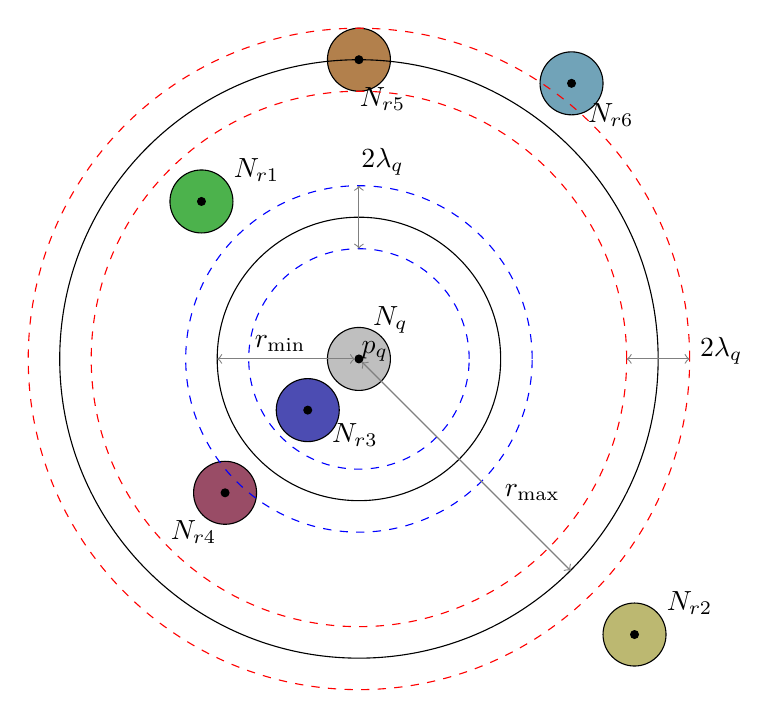
\begin{tikzpicture}
  % N_q
  \draw [fill=lightgray] (0, 0) circle (0.4);
  \node [ ] at (0.4, 0.5) { $\mathscr{N}_q$ };

  % p_q
  \node [draw, circle, inner sep=1pt, fill] at (0, 0) { };
  \node [ ] at (0.2, 0.1) { $p_q$ };

  % N_{r1}
  \draw [fill=green!40!gray] (-2.0, 2.0) circle (0.4);
  \node [draw, circle, inner sep=1pt, fill] at (-2.0, 2.0) { };
  \node [ ] at (-1.3, 2.4) { $\mathscr{N}_{r1}$ };

  % N_{r2}
  \draw [fill=yellow!40!gray] (3.5, -3.5) circle (0.4);
  \node [draw, circle, inner sep=1pt, fill] at (3.5, -3.5) { };
  \node [ ] at (4.2, -3.1) { $\mathscr{N}_{r2}$ };

  % N_{r3}
  \draw [fill=blue!40!gray] (-0.65, -0.65) circle (0.4);
  \node [draw, circle, inner sep=1pt, fill] at (-0.65, -0.65) { };
  \node [ ] at (-0.05, -0.97) { $\mathscr{N}_{r3}$ };

  % N_{r4}
  \draw [fill=purple!40!gray] (-1.7, -1.7) circle (0.4);
  \node [draw, circle, inner sep=1pt, fill] at (-1.7, -1.7) { };
  \node [ ] at (-2.1, -2.2) { $\mathscr{N}_{r4}$ };

  % N_{r5}
  \draw [fill=orange!40!gray] (0, 3.8) circle (0.4);
  \node [draw, circle, inner sep=1pt, fill] at (0, 3.8) { };
  \node [ ] at (0.3, 3.3) { $\mathscr{N}_{r5}$ };

  % N_{r6}
  \draw [fill=cyan!40!gray] (2.7, 3.5) circle (0.4);
  \node [draw, circle, inner sep=1pt, fill] at (2.7, 3.5) { };
  \node [ ] at (3.2, 3.1) { $\mathscr{N}_{r6}$ };

  % l
  \draw (0, 0) circle (1.8);
  % l - \lambda_q
  \draw [blue, dashed] (0, 0) circle (1.4);
  % l + \lambda_q
  \draw [blue, dashed] (0, 0) circle (2.2);

  % u
  \draw (0, 0) circle (3.8);
  % u - \lambda_q - \lambda_r
  \draw [red, dashed] (0, 0) circle (3.4);
  % u + \lambda_q + \lambda_r
  \draw [red, dashed] (0, 0) circle (4.2);

  % line from p_q to l
  \draw [gray, arrows=<->] (-0.05, 0) -- (-1.8, 0);
  \node [ ] at (-1.0, 0.2) { $r_{\min}$ };

  % line from p_q to u
  \draw [gray, arrows=<->] (0.04, -0.04) -- (2.687, -2.687);
  \node [ ] at (2.2, -1.7) { $r_{\max}$ };

  % line indicating u shell
  \draw [gray, arrows=<->] (4.2, 0) -- (3.4, 0);
  \node [ ] at (4.6, 0.1) { $2\lambda_q$ };

  % line indicating l shell
  \draw [gray, arrows=<->] (0, 2.2) -- (0, 1.4);
  \node [ ] at (0.3, 2.5) { $2 \lambda_q$ };

\end{tikzpicture}

%\caption{The shape of geometry to come.}
%\label{fig:rs_shapes}
%\end{centering}
%\end{figure}

%Figure \ref{fig:rs_shapes} details the possibilities when a particular
%combination is visited.

%\begin{enumerate}
%\item If the reference node is entirely contained in the range $[l +
%\lambda_q, u - \lambda_q]$ (as in $\mathscr{N}_{r1}$), then every
%descendant point of the reference node will be in the results for every
%descendant point of the query node; these can be added and then the combination
%can be pruned.\footnote{Because we have assumed that each query point will have
%$O(1)$ results, the total runtime of this step for each query node is $O(1)$, or
%$O(N)$ during the whole algorithm.  We will not consider the runtime
%contribution of this situation further, because other factors will outweigh
%this.}

%\item If the reference node is not contained at all in the range $[l -
%\lambda_q, u + \lambda_q]$ (as in $\mathscr{N}_{r2}$ and
%$\mathscr{N}_{r3}$), then no descendant points of the reference node will be in
%the results for any descendant point of the query node; thus, the combination
%can simply be pruned.

%\item If the reference node overlaps with the ranges $[l - \lambda_q,
%l + \lambda_q]$ or $[u - \lambda_q, u + \lambda_q]$ (as in
%$\mathscr{N}_{r4}$, $\mathscr{N}_{r5}$, and $\mathscr{N}_{r6}$), the node
%combination cannot be pruned by \texttt{Score()}, and must be descended.  This
%is the interesting case that we will focus on hereafter.  Only combinations of
%this type will make up the reference nodes in $|R_r^*|$.
%\end{enumerate}

%In the last situation, a reference node $\mathscr{N}_r$ with center $p_r$ and
%furthest descendant distance $\lambda_r$ satisfies at least one of the following
%two conditions:

%\begin{eqnarray}
%p_r &\in& B_{S_r}(p_q, u + \lambda_q + \lambda_r) \setminus B_{S_r}(p_q, u -
%\lambda_q - \lambda_r), \\
%p_r &\in& B_{S_r}(p_q, l + \lambda_q + \lambda_r) \setminus B_{S_r}(p_q, l -
%\lambda_q - \lambda_r).
%\end{eqnarray}

%Assuming first that $l - \lambda_q - \lambda_r > 0$, the reference node lies in
%the outer shell of a ball.  This is true of any $\mathscr{N}_r \in R_r$ for any
%cover set $R_r$ during the traversal.  If we can bound the size of the set

%\begin{equation}
%\left(B_{S_r}(p_q, u + \lambda_q + \lambda_r) \setminus B_{S_r}(p_q, u -
%\lambda_q - \lambda_r) \right) \cup \left(B_{S_r}(p_q, l + \lambda_q +
%\lambda_r) \setminus B_{S_r}(p_r, l - \lambda_q - \lambda_r) \right)
%\end{equation}

%\noindent then we will have bounded $| R_r^* |$.  First, observe that $\lambda_q
%+ \lambda_r \le 2^{s_r^{\max} + 1}$; then, the following algebraic
%manipulations lead us to our result.

%\begin{cor}
%In the monochromatic case ($S_q = S_r$, and $c_r = c_{qr} = c$), the
%running time of range search or range count is bounded by $O(c^{8 + \beta} N)$.
%\end{cor}

In this setting we can more easily consider the relation of the running time to
$\alpha$.  Consider $\alpha = (1 / 3)$; this yields a running time of $O(c^8 (N
+ \theta))$.  $\alpha = (1 / 7)$ yields $O(c^9 (N + I_t(\mathscr{N}_q +
\theta))$, $\alpha = (1 / 15)$ yields $O(c^{10} (N + I_t(\mathscr{N}_q) +
\theta))$, and so forth.  As $\alpha$ gets smaller, the exponent on $c$ gets
larger, and diverges as $\alpha \to 0$.

For reasonable runtime it is necessary that the $\alpha$-expansion of $S_{\max}$
be bounded.  This is because the dual-tree recursion must retain reference nodes
which may contain descendants in the range set $S[p_q]$ for some query $p_q$.
The parameter $C$ of the $\alpha$-expansion allows us to bound the number of
reference nodes of this type, and if $\alpha$ increases but $C$ remains small
enough that Corollary \ref{cor:rs} applies, then we are able to obtain tighter
running bounds.

%The assumption that on number of points in the range of $[(1 - \alpha)l, (1 +
%\alpha)u]$ for a single query is not too restrictive, but must be satisfied for
%the result to be meaningful.  After all, if that assumption is not satisfied,
%then it is not possible to perform range search in $O(1)$ time for each query
%point, making an $O(N)$ bound for the whole query set impossible.

%To show where the assumption is valid, consider that when presented with a very
%large dataset, a practitioner may perform monochromatic range search on a range
%$[l, u]$ for a geometric subset of their data; for instance, a hypersquare
%with side length $2u$.  This might be done in order to find a range $[l, u]$
%that produces a manageable number of results (if the range is too large, the
%number of results returned for each query point may be enormous).  Then, that
%practitioner may scale to a larger dataset by simply increasing the size of
%their hypersquare.  In this setting, the number of points in the range of
%$[(1 - \alpha)l, (1 + \alpha)u]$ for a single query remains $O(1)$ with respect
%to $N$.  Alternately, it should be possible to tighten the range $[l, u]$ as $N$
%increases in such a way that the number of points in the range remains constant.

%In cases where this assumption is not thought to be valid, it is straightforward
%to prove a bound on the running time of range search or range count by using the
%aspect ratio of the data, as in \cite{curtin2014kernel}.  However, the aspect
%ratio is particularly sensitive to datasets that have arbitrarily close points,
%and it is difficult to make assumptions about the aspect ratio.

%Alternately, if the assumption is not valid but it can be shown that the number
%of points in the range $[(1 - \alpha)l, (1 + \alpha)u]$ is $O(k)$ where $k$ has
%some dependence on $N$, then the running time can be easily bounded as $O(c^{4 +
%\beta} k(N + \theta))$.

%Also, note that the proof considers points with distance from $p_q$ in
%the range $[l + \lambda_q + \lambda_r, u - \lambda_q - \lambda_r]$; however, the
%pruning rule could also prune points that lie entirely in the range $[l, u]$ for
%additional speedup (Algorithm \ref{alg:rs_sc} does not do this because there is
%no theoretical benefit in our proof).  Unfortunately, the expansion constant
%does not make working with slices of balls easy, and as a result the runtime
%bound as given is likely to be loose when this additional prune is made,
%especially when $u - l$ is large.
